\documentclass[19pt,a4paper]{article}
\usepackage{xeCJK}
\usepackage{amsmath}
\setmainfont{STSong}
\usepackage{geometry}
\geometry{left=2.5cm,right=2.5cm,top=2.5cm,bottom=2.5cm}
\setlength{\parindent}{4em}
\title{思考题5——有限空间选择和排序}
\author{孟妍廷\quad 2015202009}
\date{2017年10月24日}

\begin{document}
\maketitle

首先对题目的几个理解:\\
\indent 1.只读数组:只能获取值而不能被赋值的数组,因此一定需要额外空间才能进行选择和排序\\
\indent 2. k为1到n的值,但是由于对称性我们可以假设$k\le\lceil\frac{n}{2}\rceil$.因为当k超过n的一半的时候\\
\indent 相当于求第n-k小的数,而n-k小于n的一半,逻辑仍然相同.\\
\indent 1.读取一遍,选择第k大的数需要的额外空间至少为$\Omega(n)>\Omega(k)$,只有当k为中位数或非常接近\\
\indent 中位数时,额外空间为$\Theta(n^{\frac{1}{2}})<O(\frac{n}{2})=O(k)$,以任意高的可能性找到k.\\
\indent 通过阅读文献,证明如下:\\
\indent 不失一般性,假设额外空间大小为s.算法将第一个s读入内存,并决定在读取第s+1个时丢弃\\
\indent 哪一个."敌人策略"确保第s+1个元素进入时不影响被替代的元素之外的所有元素的顺序.\\
\indent 重复"敌人策略",当$x=\lfloor\frac{n}{2s-1}\rfloor$时,第$sx+1$个元素正准备被读入,此时内存中起码有一个位\\
\indent  置被替换出去的元素组成一个集合X,其中至少有x个元素未被比较过且未被排序.可以证明\\
\indent 剩余的n-sx个元素的中位数可以被设计为X的中位数.因此每次丢弃s个元素产生的未被比较\\
\indent 的集合大小最多为$\lceil\frac{n}{s}\rceil$.因此辅助定理3可证。\\
\begin{figure}[htbp]
 \centering
 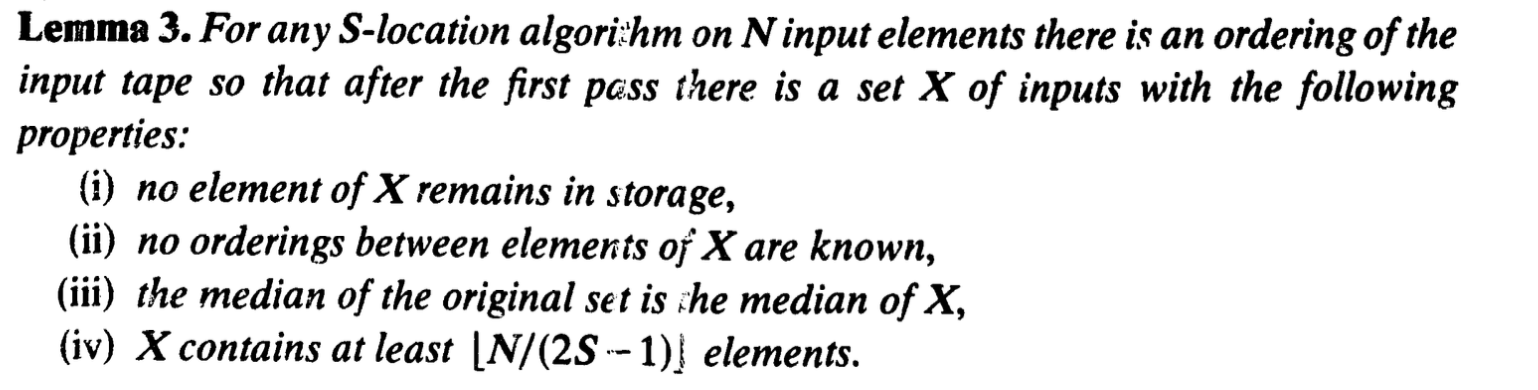
\includegraphics[scale=0.4]{1.png}
\end{figure}\\
\indent 由辅助定理3可以证明定理4:\\
\begin{figure}[htbp]
 \centering
 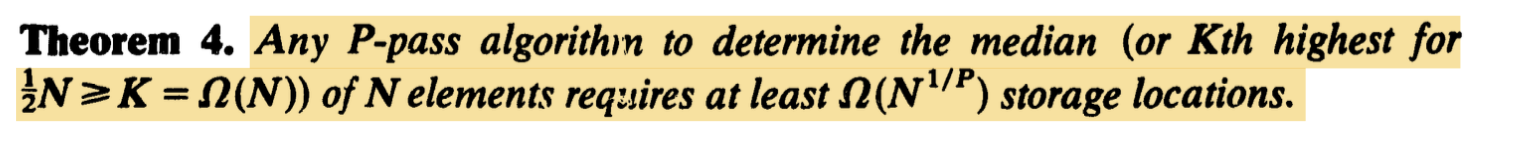
\includegraphics[scale=0.4]{2.png}
\end{figure}\\
\indent 此时p为1,因此平均情况需要的额外空间至少为$\Omega(n)$,只有在第k大的元素正好位于k处时\\
\indent 才能达到$\Omega(k)$\\
\indent 而当k为中位数时,由于为选择合适的额外存储空间s,要求当前位于s中的s-1个元素是连续的\\
\indent 并尽可能接近当前的中值,因此有定理5:\\
\begin{figure}[htbp]
 \centering
 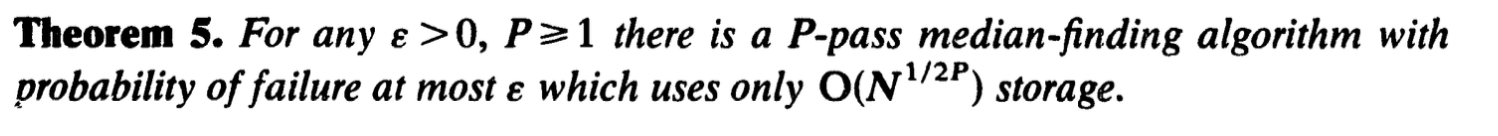
\includegraphics[scale=0.4]{3.png}
\end{figure}\\
\indent 此时p为1,得证。\\
\\
\indent 2.至少需要$\Omega(n^\frac{1}{2})$,至多需要$O(n^\frac{1}{2}logn)$的额外空间。\\
\indent 由1.中的定理4可知当p=2时,额外空间至少为$\Omega(n^\frac{1}{2})$.\\
\\
\\
\\
\\
\\
\\
\indent 又由辅助定理1可得\\
\begin{figure}[htbp]
 \centering
 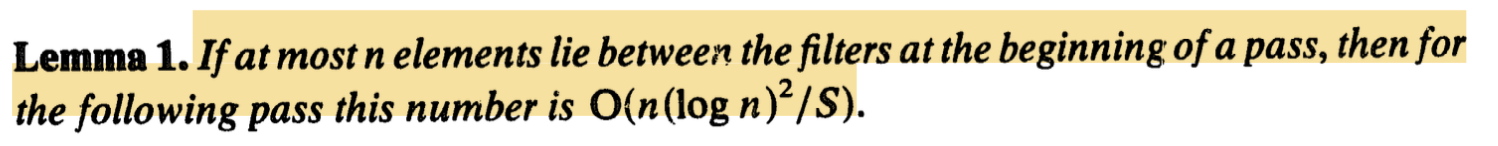
\includegraphics[scale=0.4]{4.png}
\end{figure}\\
\indent 可以推出定理2\\
\begin{figure}[htbp]
 \centering
 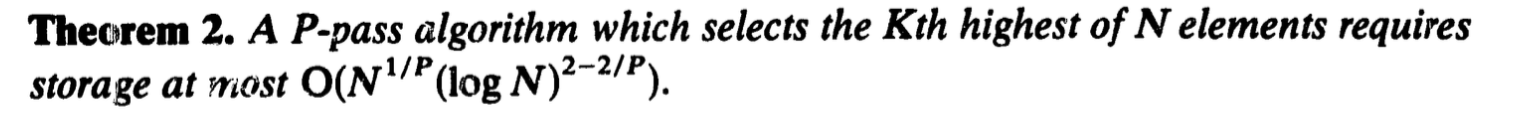
\includegraphics[scale=0.4]{5.png}
\end{figure}\\
\indent 此时p=2,得证。\\
\indent 设计算法如下:\\
\indent $sort(A,k)$\\
\indent $len\ =\ \lceil sqrt(A.length)\rceil$\\
\indent $B[len]\ =\ {0}\ \ \ 初始化$\\
\indent $for\ i=0\ to\ len-1$\\
\indent $\ \ \ \ B[i]=A[i]\ \ \ 放入A的前len个元素$\\
\indent $while(i<A.length)$
\indent $\ \ \ \ for\ j=i\ to\ i+len-1$\\
\indent $\ \ \ \ \ \ \ \ 用A中后len个元素中比B[0...len-1]中元素小的替换它们$\\
\indent $\ \ \ \ \ \ \ \  用排序算法对B排序$\\
\indent $\ \ \ \ i++$\\
\indent 由此可以得到第len大的数,若len>=k已经得到结果,如果len<k,则以第len大的数为B[0]\\
\indent 重复以上步骤,直至找到第k大的数,该算法的空间复杂度为$\Omega(n^{\frac{1}{2}})$\\











\end{document}